\begin{definition}[Measurable space]
    A \textit{measurable space} is a tuple $(X, \mathcal{A})$, where:
    \begin{enumerate}
        \item {
            $X$ is a set.
        }
        \item {
            $\mathcal{A}$ is a $\sigma$-algebra on $X$.
        }
    \end{enumerate}
\end{definition}

\begin{definition}[Measure space]
    A \textit{measure space} is a triple $(X, \mathcal{A}, \mu)$, where:
    \begin{enumerate}
        \item {
            $X$ is a set.
        }
        \item {
            $\mathcal{A}$ is a $\sigma$-algebra on $X$.
        }
        \item {
            $\mu$ is a measure on $(X, \mathcal{A})$.
        }
    \end{enumerate}
\end{definition}

\begin{example}[1]
    $\{\emptyset, X\}$ is a $\sigma$-algebra. Any $\mu$, such that
    $\mu(\emptyset) = 0$ and $\mu(X) \ge 0$ will be a measure.
\end{example}
\begin{example}[2]
    $2^X$ is a $\sigma$-algebra. We can have the following measures:
    \begin{enumerate}[label=\alph*)]
        \item {
            $\mu(E) = \abs{E}$ is called a \textit{counting measure}.
            Here $\abs{E}$ denotes the cardinality of $E$ (number of elements in $E$).
        }
        \item {
            $\delta$-measure (also called Dirac measure):
            \[
                \mu(E) = \begin{cases}
                    1, &0 \in E\\
                    0, &\text{otherwise}
                \end{cases}
            \]
        }
    \end{enumerate}
\end{example}

\subsection{Continuity of measure}

\begin{definition}
    A countable collection of sets $\{E_k\}_{k=1}^\infty$ is called
    \textit{ascending} if $E_k \subset E_{k+1}$.
\end{definition}
\begin{definition}
    A countable collection of sets $\{E_k\}_{k=1}^\infty$ is called
    \textit{descending} if $E_k \supset E_{k+1}$.
\end{definition}

\begin{theorem}[Continuity of measure]
    \label{the:continuityOfMeasure}
    \mbox{}
    \begin{enumerate}
        \item {
            If $\{A_k\}_{k=1}^\infty \subset \mathcal{A}$ and the sequence is ascending,
            then
            \[
                \mu\Bigl(\bigcup_{k=1}^\infty A_k\Bigr) = \lim_{k \to \infty} \mu(A_k)
            \]
        }
        \item {
            If $\{B_k\}_{k=1}^\infty \subset \mathcal{A}$, the sequence is descending and $\mu(B_1) < \infty$,
            then
            \[
                \mu\Bigl(\bigcap_{k=1}^\infty B_k\Bigr) = \lim_{k \to \infty} \mu(B_k)
            \]
        }
    \end{enumerate}
\end{theorem}
\begin{proof}
    \begin{enumerate}
        \item {
            Let $C_k \coloneqq A_k \setminus A_{k-1}$. Then we have:

            \begin{figure*}[h]
                \centering
                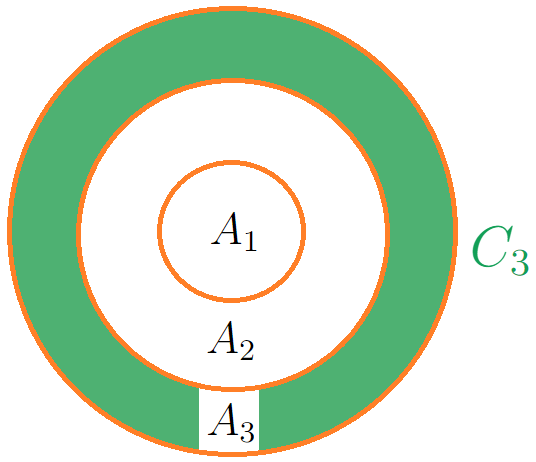
\includegraphics[width=0.3\textwidth]{a1a2a3}
            \end{figure*}

            \[
                \mu\Bigl(\bigcup_{k=1}^\infty A_k\Bigr) =
                \mu\Bigl(\bigsqcup_{k=1}^\infty C_k\Bigr) =
                \sum_{k=1}^\infty \mu(C_k) =
                \lim_{n \to \infty} \sum_{k=1}^n \mu(C_k) = \lim_{n \to \infty} \mu(A_n)
            \]
        }
        \item {
            Let $D_k \coloneqq B_1 \setminus B_k$. 
            Since $B_k$ is descending, it follows that $D_k$ is an ascending sequence. Then from the part 1 of the theorem it follows that:
            \begin{align*}
                &
                \mu\Bigl(\bigcup_{k=1}^\infty D_k\Bigr) = \lim_{k \to \infty} \mu(D_k)
                \qquad
                \bigcup_{k=1}^\infty D_k = B_1 \setminus \bigcap_{k=1}^\infty B_k
                \\&
                \mu\Bigl(B_1 \setminus \bigcap_{k=1}^\infty B_k\Bigr) =
                \lim_{k \to \infty}\bigl(\mu(B_1) - \mu(B_k)\bigr) =
                \mu(B_1) - \lim_{k \to \infty} \mu(B_k)
                \\&
                \mu\Bigl(B_1 \setminus \bigcap_{k=1}^\infty B_k\Bigr) =
                \mu(B_1) - \mu\Bigl(\bigcap_{k=1}^\infty B_k\Bigr) \implies
                \mu\Bigl(\bigcap_{k=1}^\infty B_k\Bigr) = \lim_{k \to \infty} \mu(B_k)
            \end{align*}
        }
    \end{enumerate}    
\end{proof}

\begin{definition}
    We say that a statement (property) holds for \textit{almost all} $x \in X$
    \textit{with respect to a measure $\mu$}, if
    $\exists N \in \mathcal{A}$, such that $\mu(N) = 0$ and the statement (property)
    holds for all $x \in X \setminus N$.
\end{definition}
\begin{lemma}[Borel–Cantelli]
    Let $(X, \mathcal{A}, \mu)$ be a measure space. Let
    $\{E_k\}_{k=1}^\infty \subset \mathcal{A}$ and $\sum_{k=1}^\infty \mu(E_k) < \infty$.
    Then \textit{almost all} $x \in X$ belong to at most finitely many $E_k$.
\end{lemma}
\begin{proof}
    Let $B_n = \cup_{k=n}^\infty E_k$. It's easy to see that $B_k$ is a descending measure.
    At the same time,
    \[ \mu(B_1) = \mu\Bigl(\bigcup_{k=1}^\infty E_k\Bigr) \le \sum_{k=1}^\infty \mu(E_k) < \infty \]
    By definition of $B_n$, $\cap_{n=1}^\infty B_n$ contains all the points
    that are contained in infinitely many $E_k$'s. But, by \hyperref[the:continuityOfMeasure]{continuity of measure} 
    for $\{B_n\}_{n=1}^\infty$ we have:
    \[ 
        \mu\Bigl(\bigcap_{n=1}^\infty B_n\Bigr) =
        \lim_{n \to \infty} \mu(B_n) =
        \lim_{n \to \infty} \Bigl(\bigcup_{k=n}^\infty E_k\Bigr) \le
        \lim_{n \to \infty} \sum_{k=n}^\infty \mu(E_k) = 0
    \]
\end{proof}

\subsection{How large is the Lebesgue $\sigma$-algebra $\mathcal{M}$?}
\begin{proposition}
    \label{prop:intervalsAreMeasurable}
    Every interval is Lebesgue-measurable.
\end{proposition}
\begin{proof}
    Proof idea:
    \[ 
        E \in \mathcal{M} \Longleftrightarrow 
        \forall A: m(A) = m(A \cap E) + m(A \cap E^C)
    \]
    Assume $E = (-\infty, a)$. If we prove that such intervals lie in $\mathcal{M}$, 
    then we'll prove everything (since $\mathcal{M}$ is a $\sigma$-algebra).
    We already have $m(A) \le m(A \cap E) + m(A \cap E^C)$ from \hyperref[the:countableSubadditivity]{countable subadditivity}.

    Let's assume $a \not\in A$ (since removing one point does not change the measure).
    Every cover of $A$ can be split into two covers with the same sum of interval lengths: of
    $A \cap (-\infty, a)$ and $A \cap (a, +\infty)$. Every interval in those
    covers, that contains $a$, can be split into two. Therefore,
    from the \hyperref[def:lebesgueOuterMeasure]{definition of Lebesgue measure}, 
    $m(A) \ge m(A \cap E) + m(A \cap E^C)$, so we've proved the inequality in both sides.
\end{proof}